Known function, simulate input, plot fANOVA and PD, comparison

PD and fANOVA: If inputs are independent, I think for the main effects fANOVA is simply PD shifted but fANOVA answers a different question thatn PD. PD usually asks for the effect of one specific variable on the prediction. In contrast, fANOVA decomposes the entire function. It is more about a global representation and clean, isolated effects because in sum they have to recover the original function and may not overlap.

\subsubsection*{Visualization for MVN}

The plots show the classical fANOVA components for our known example from the previous sections. Classical components visualized, but in this simple example they are simply the subfunctions we can already see from looking at the function.
% include a graphic from image folder right here
% Zwei Plots nebeneinander, jeweils halbe Breite

% Input: MVN, centred, independent
\begin{figure}[htpb]
    \centering
    \begin{minipage}[t]{0.49\textwidth}
        \centering
        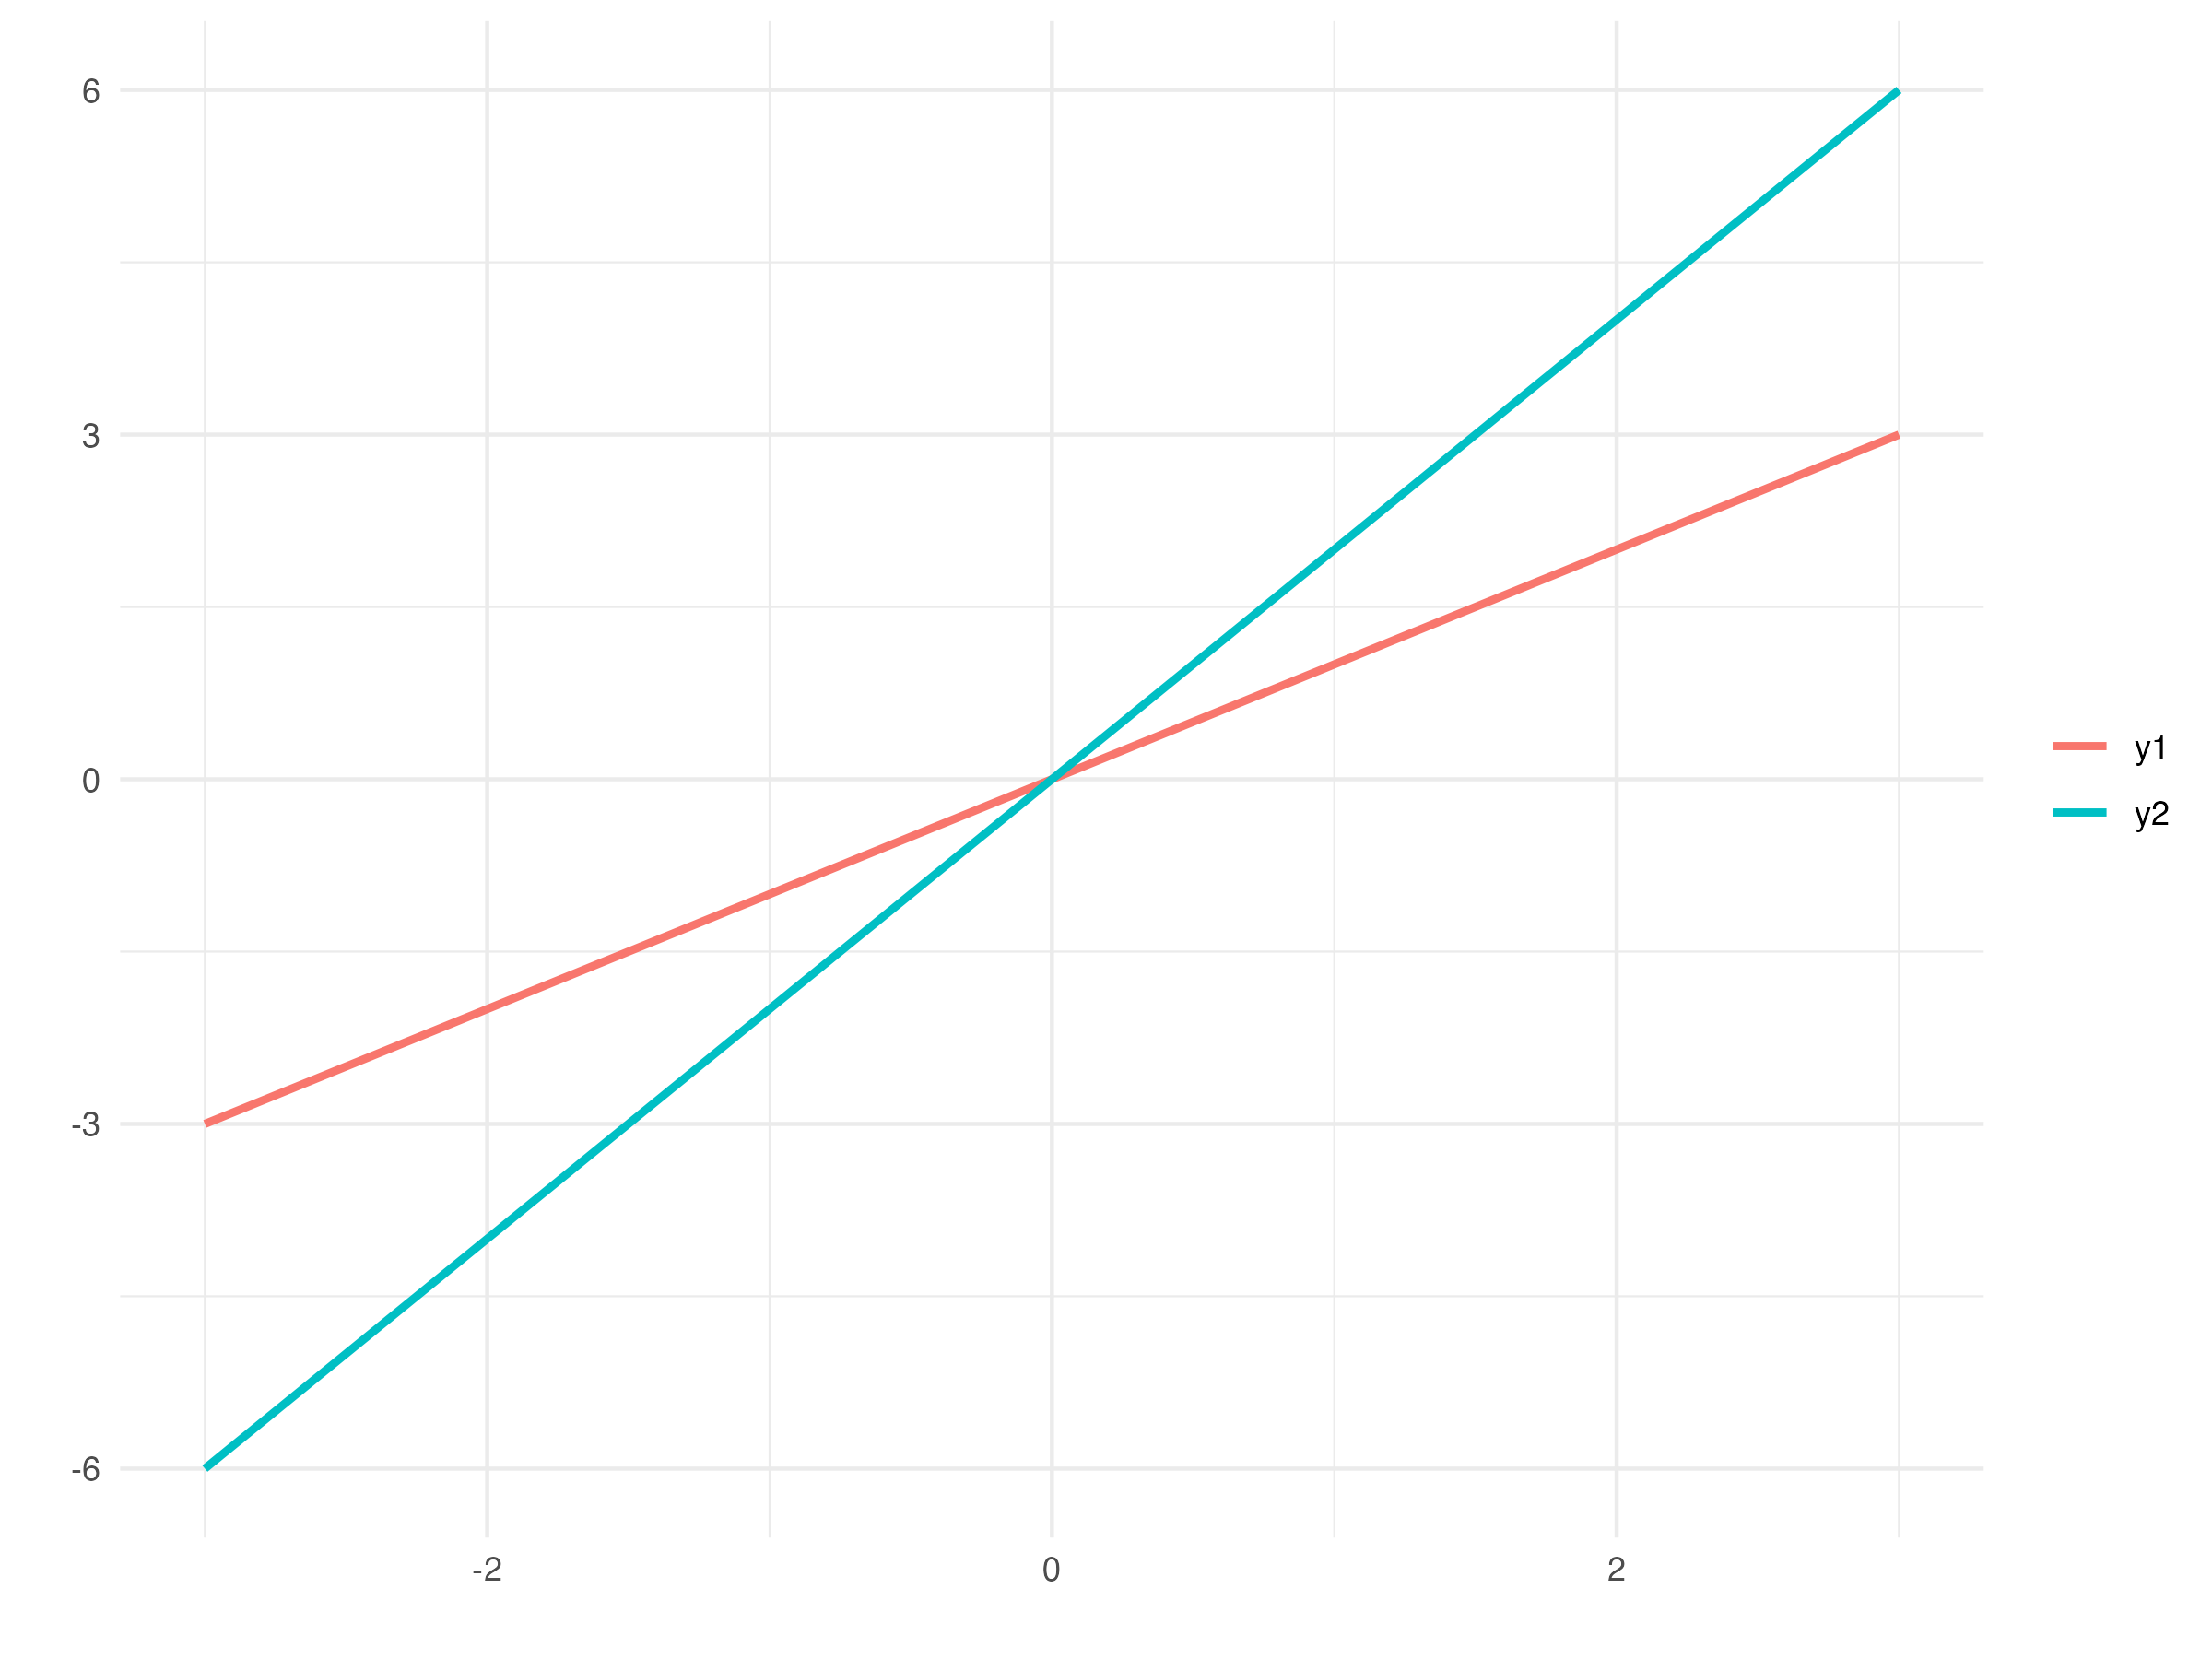
\includegraphics[width=\textwidth]{images/p_main_effect_ex1.png}
        \caption{Main terms as calculated via classical fANOVA for $g(x) = x_1 + 2 x_2 + x_1 x_2$.}
        \label{fig:main_effects_ex1}
    \end{minipage}%
    \hfill
    \begin{minipage}[t]{0.49\textwidth}
        \centering
        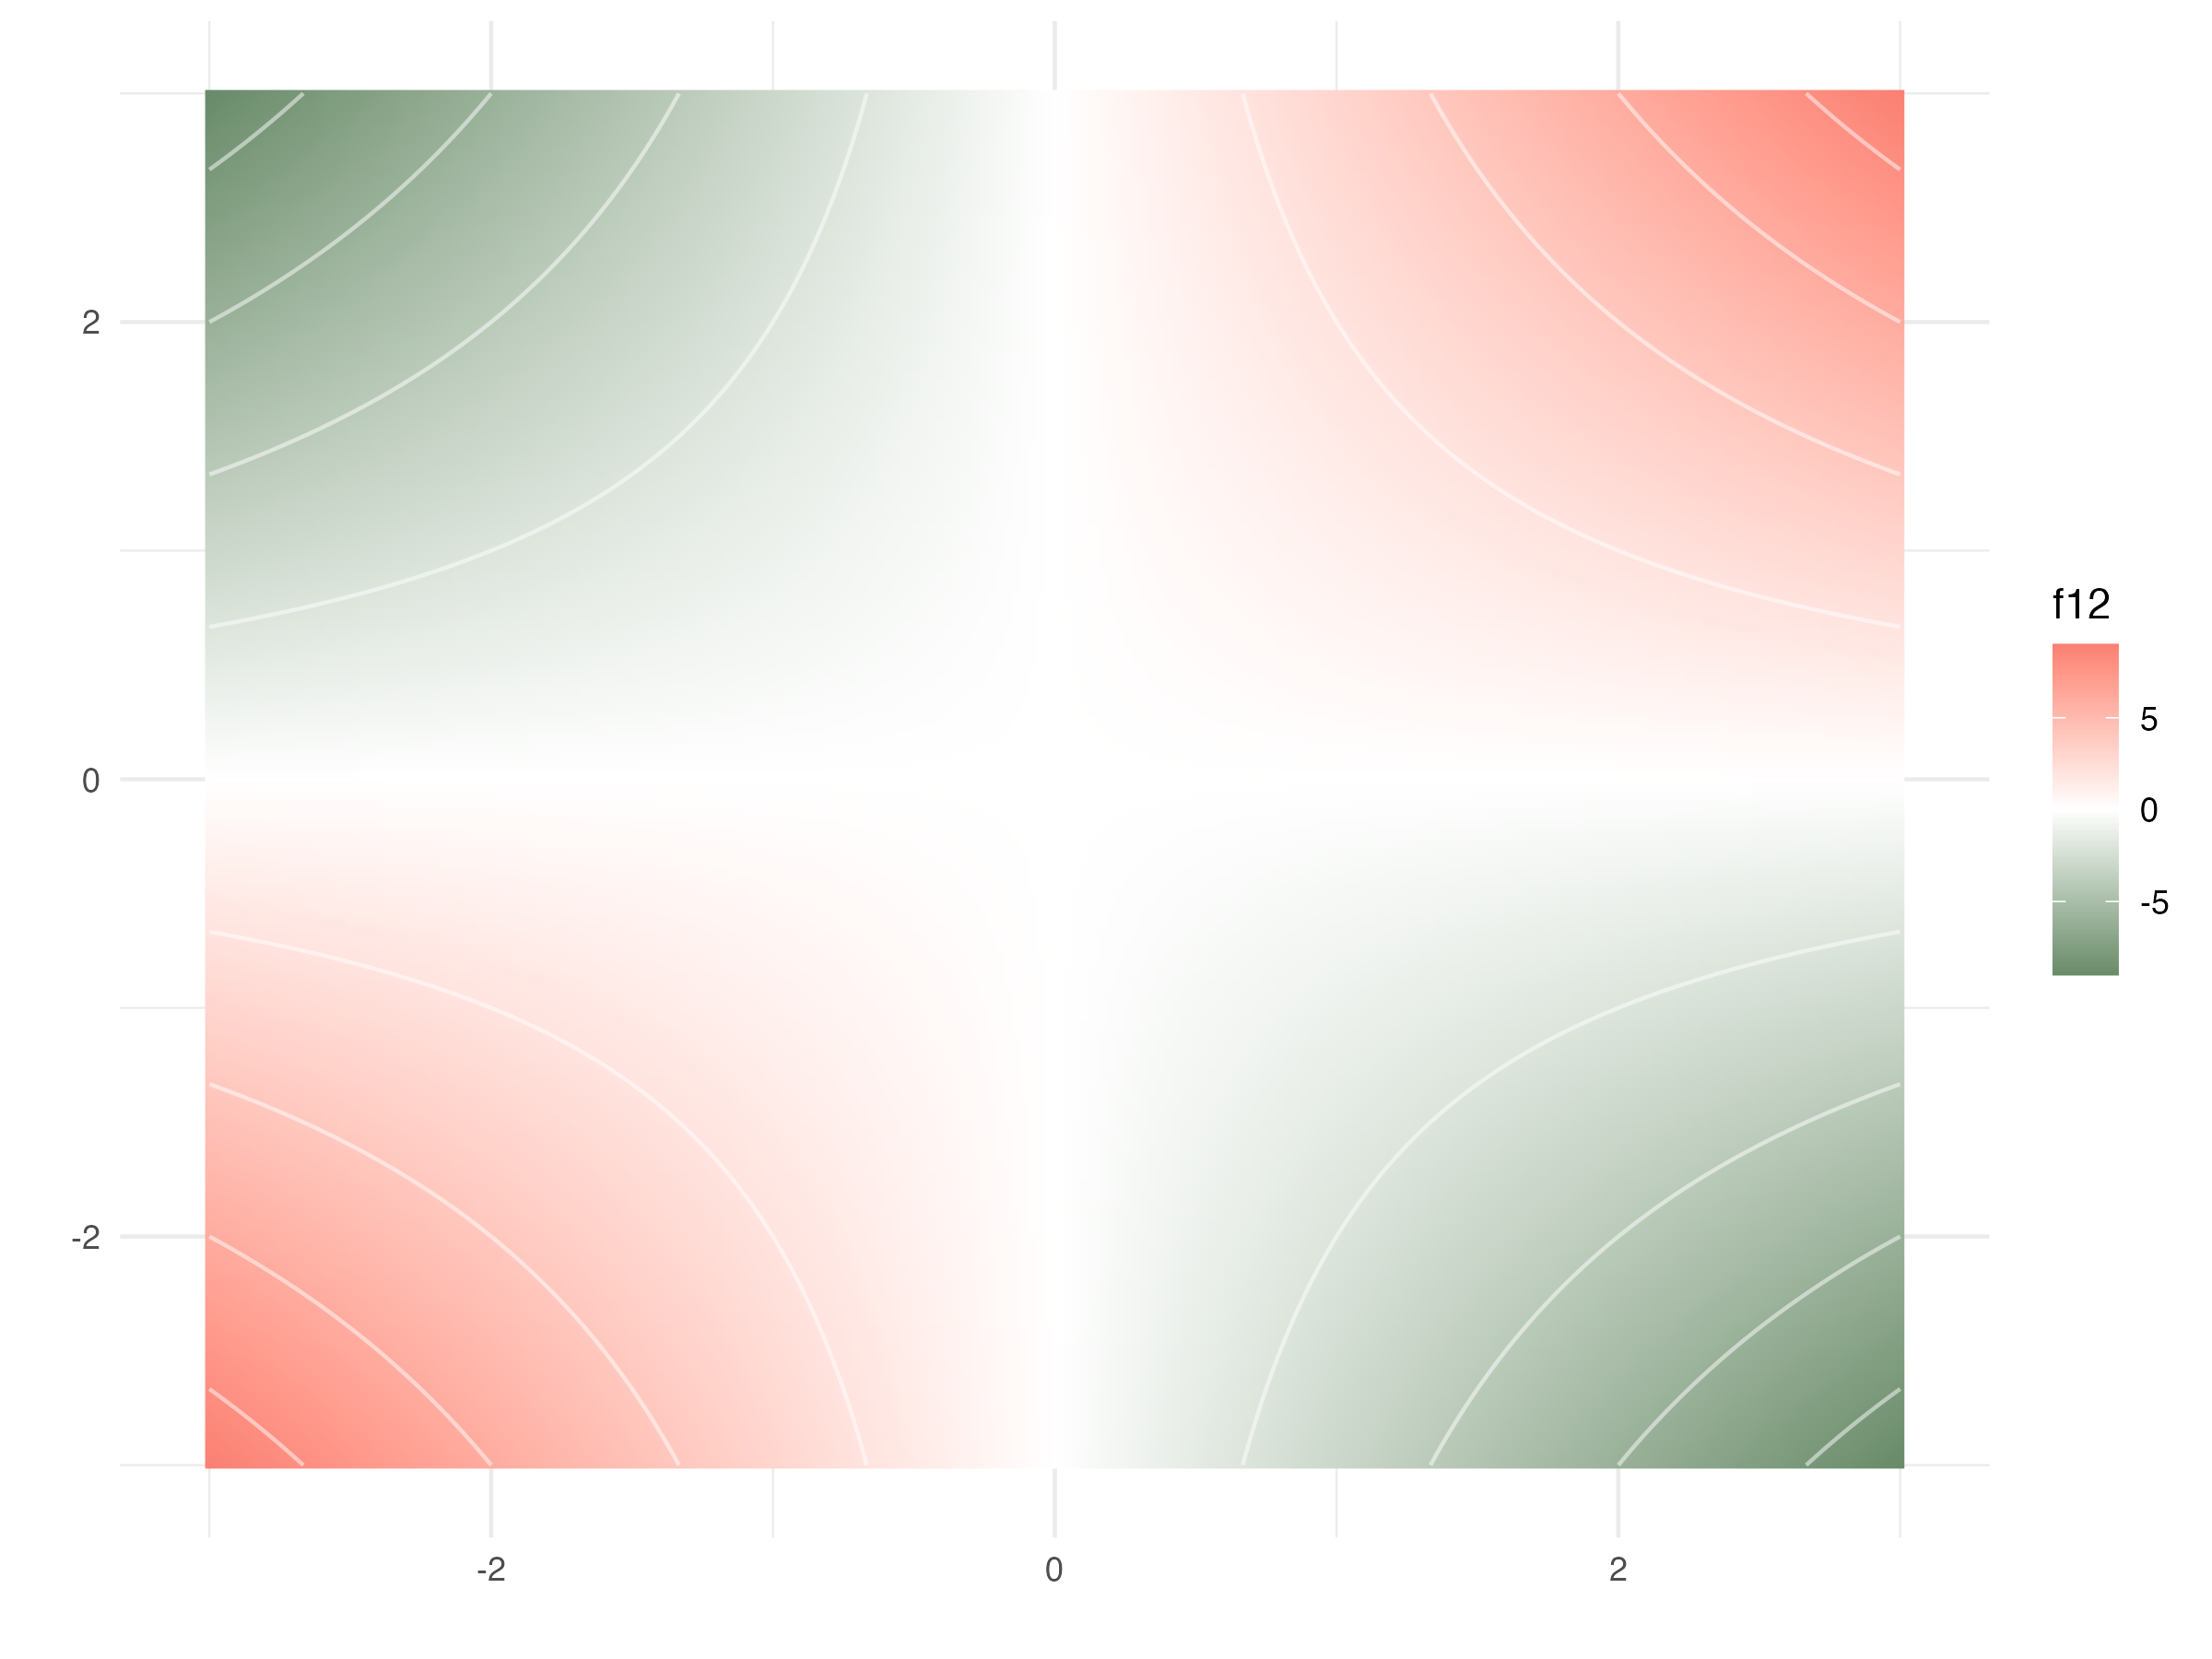
\includegraphics[width=\textwidth]{images/p_contour_ex1.png}
        \caption{Contour plot of $g(x) = x_1 + 2 x_2 + x_1 x_2$.}
        \label{fig:contour_ex1}
    \end{minipage}
\end{figure}

% Input: MVN, not centred, independent

% Input: Poisson/ Exponential/ Beta/ etc. not centred, independent


% Dependent inputs
We can compare them to the components we get under dependence from the ``naive'' approach.
% Zwei Plots für rho = 0.6 nebeneinander, jeweils halbe Breite
\begin{figure}[htpb]
    \centering
    \begin{minipage}[t]{0.49\textwidth}
        \centering
        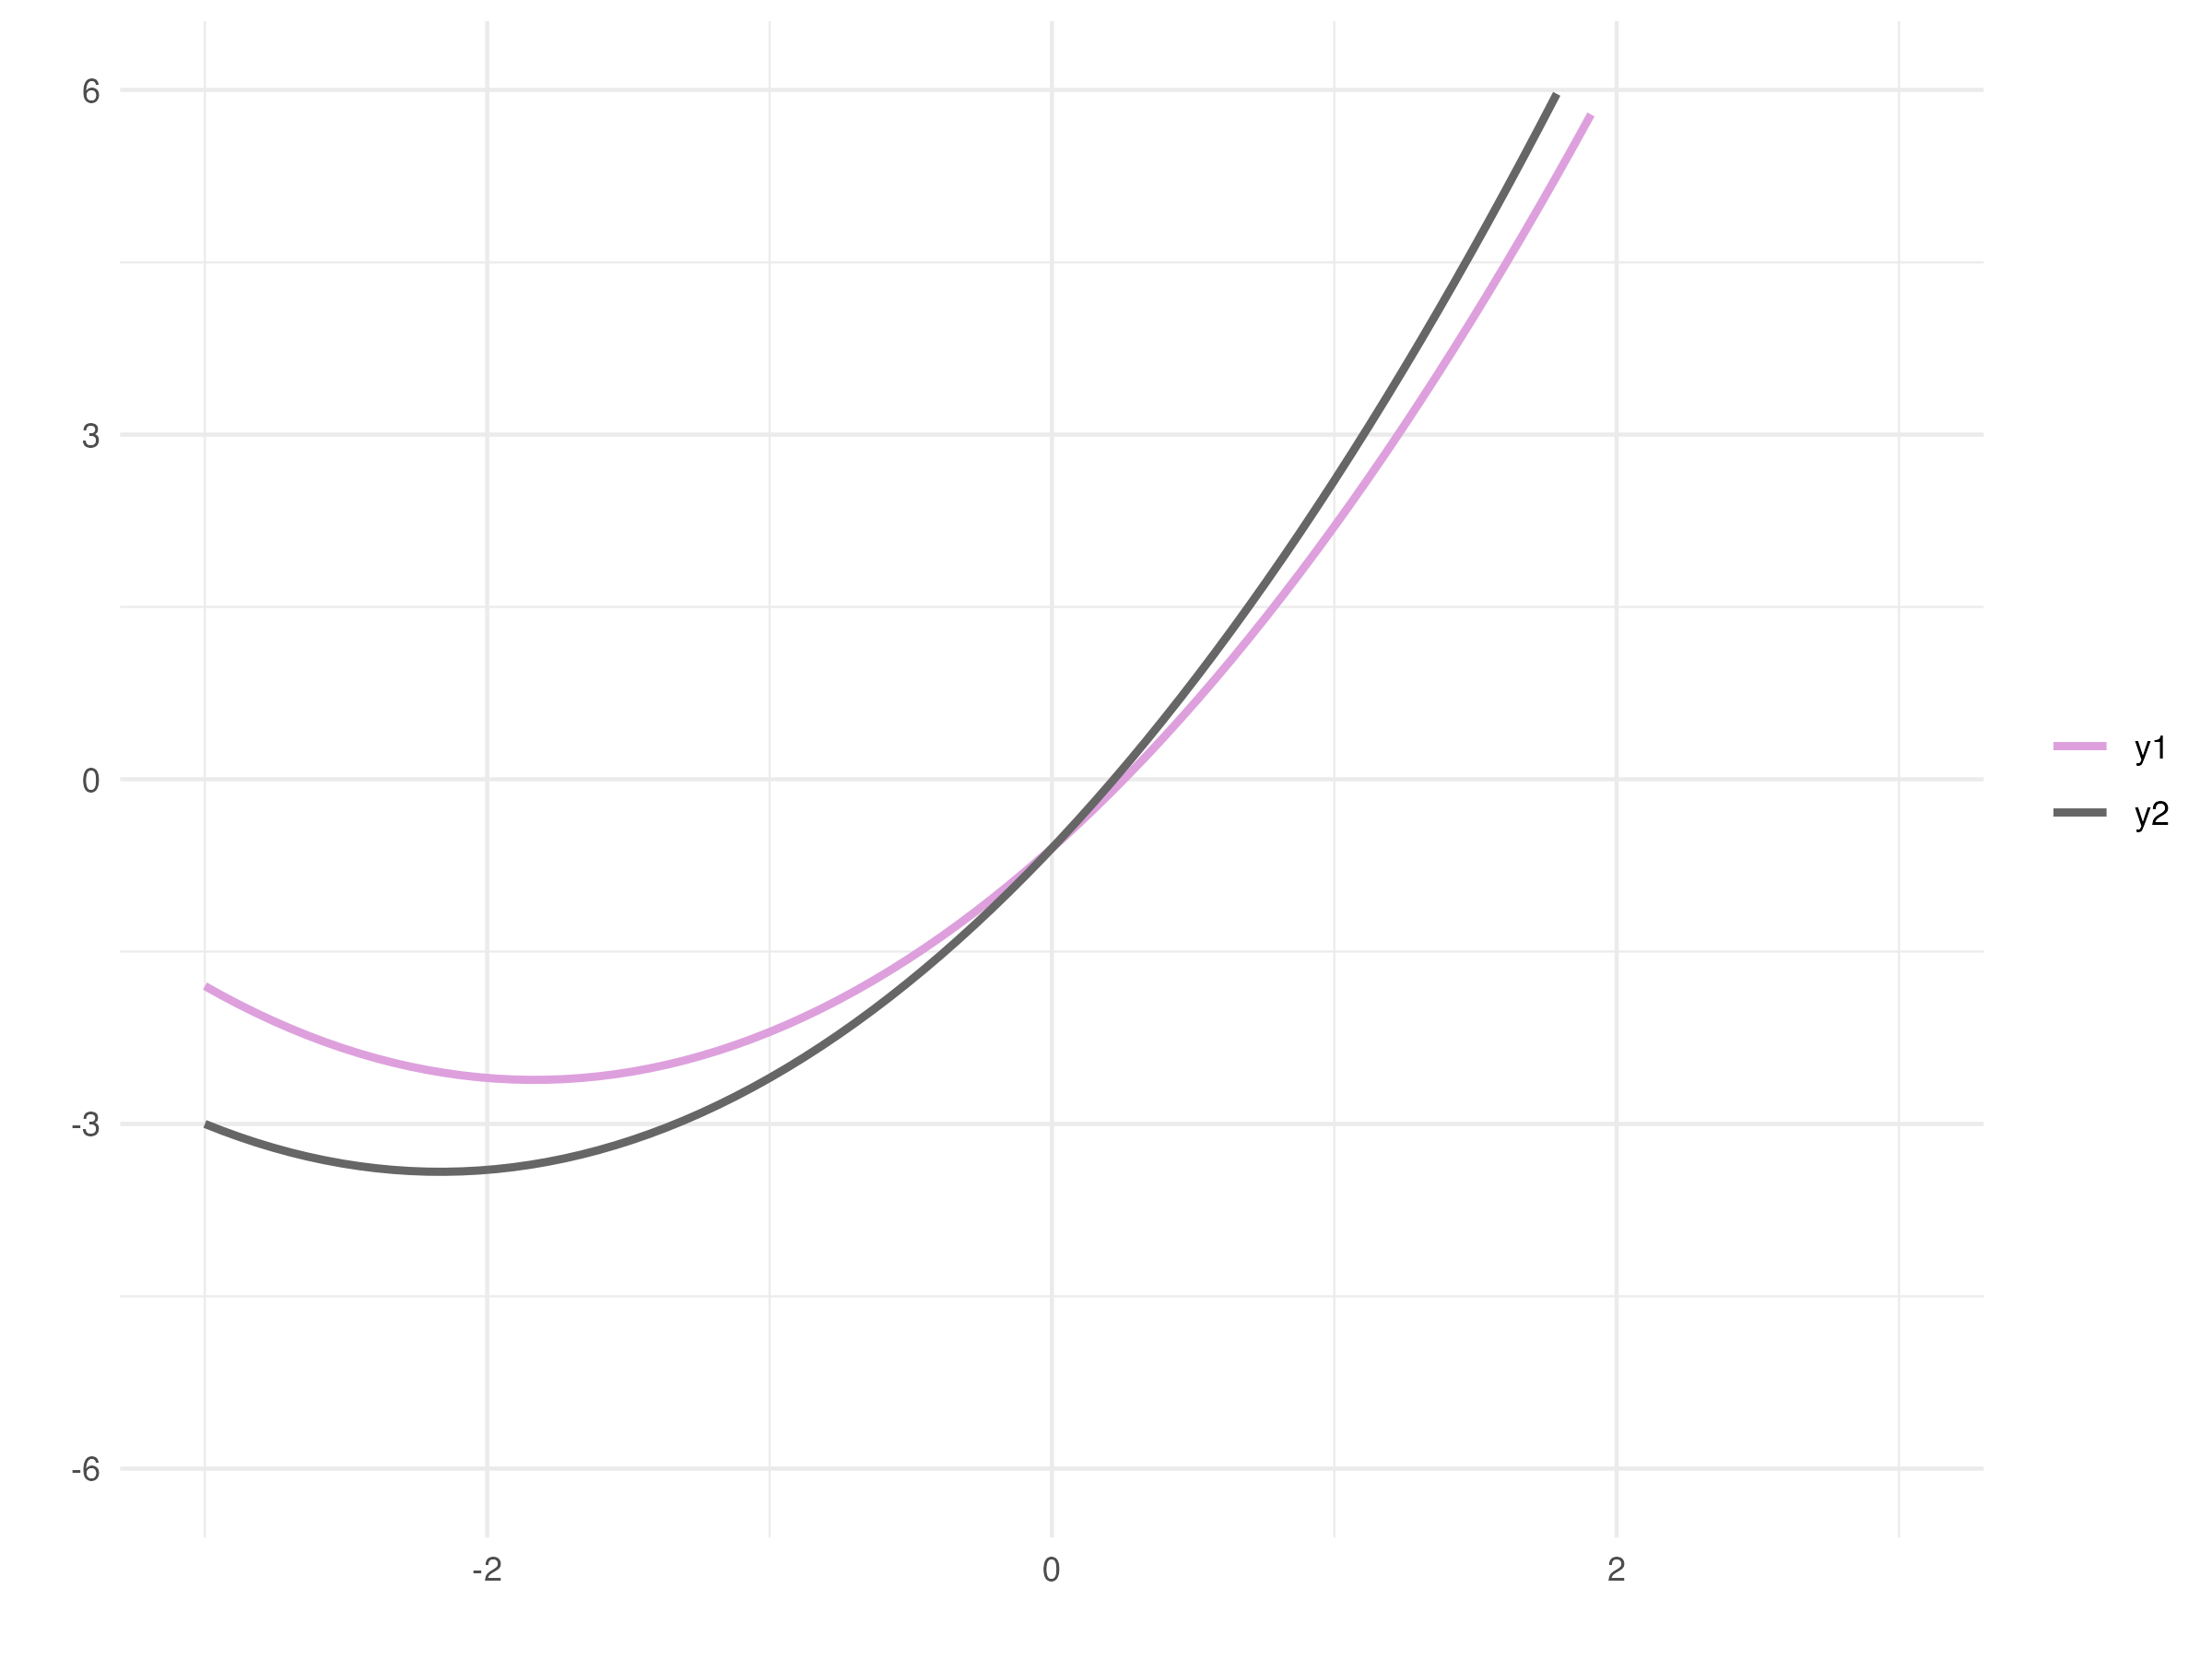
\includegraphics[width=\textwidth]{images/p_main_effect_ex1_rho06.png}
        \caption{Main terms as calculated via classical fANOVA for $g(x) = x_1 + 2 x_2 + x_1 x_2$ with $\rho = 0.6$.}
        \label{fig:main_effects_ex1_rho06}
    \end{minipage}%
    \hfill
    \begin{minipage}[t]{0.49\textwidth}
        \centering
        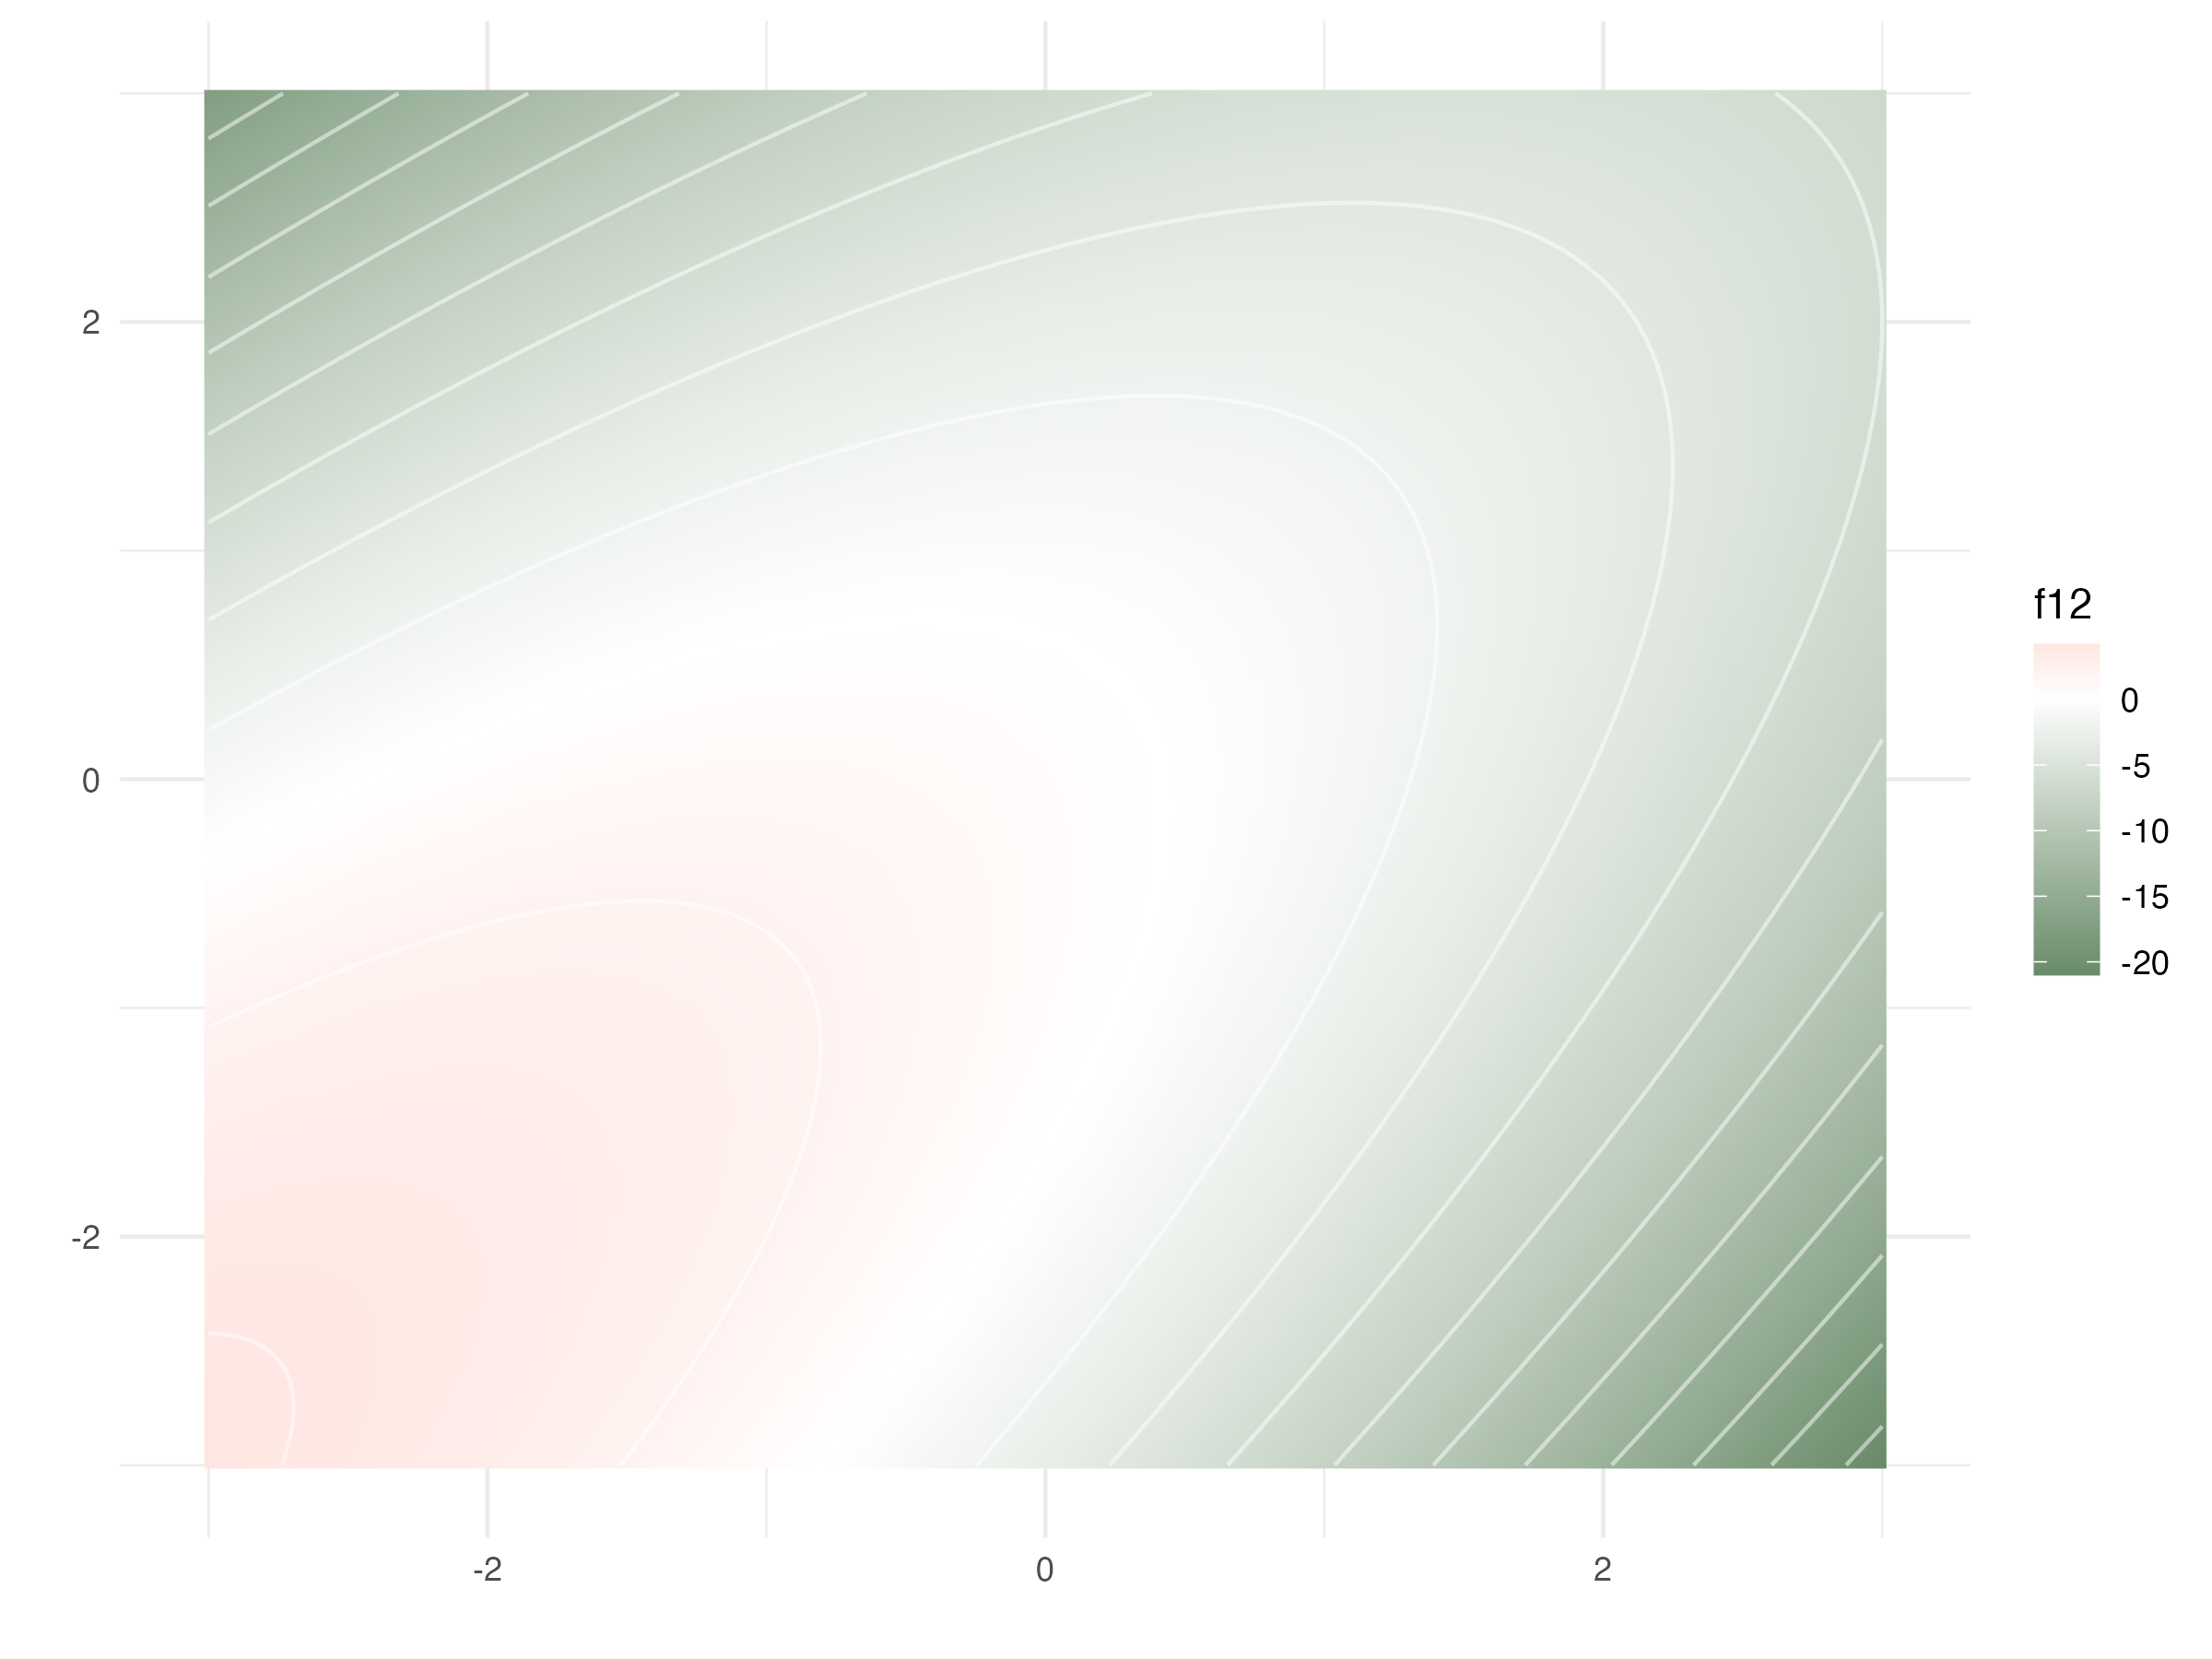
\includegraphics[width=\textwidth]{images/p_contour_ex1_rho06.png}
        \caption{Contour plot of $g(x) = x_1 + 2 x_2 + x_1 x_2$ with $\rho = 0.6$.}
        \label{fig:contour_ex1_rho06}
    \end{minipage}
\end{figure}

So \autoref{fig:main_effects_ex1_rho06} and \autoref{fig:contour_ex1_rho06} are not how we want the fANOVA components to look like under dependence - but how do we want them to look like?
Since we changed nothing about the structure of the function, should they generate identical plots as the classical components??

But on the other hand it cannot be that they give the same plots... I mean we wrote down the definition of the generalized components earlier, of course it is not the same as for the classical components. So as a function they literally look different. We couldn't compute them exactly but we could at least write out the system of equations we have to solve/ the probem that needs to be solved.